\begin{pages}
    \begin{Rightside}
    \selectlanguage{greek}
        \beginnumbering
        \pstart[
        			\chapter{Τὸ τὴν γῆν θερίσαι}
        			\markboth{The Reaping of the Earth}
				]
		Καὶ εἶδον, καὶ ἰδοὺ τὸ Ἀρνίον ἑστὸς ἐπὶ τὸ ὄρος Σιών, καὶ μετ’ αὐτοῦ ἑκατὸν τεσσεράκοντα τέσσαρες χιλιάδες ἔχουσαι τὸ ὄνομα αὐτοῦ καὶ τὸ ὄνομα τοῦ Πατρὸς αὐτοῦ γεγραμμένον ἐπὶ τῶν μετώπων αὐτῶν. καὶ ἤκουσα φωνὴν ἐκ τοῦ οὐρανοῦ ὡς φωνὴν ὑδάτων πολλῶν καὶ ὡς φωνὴν βροντῆς μεγάλης, καὶ ἡ φωνὴ ἣν ἤκουσα ὡς κιθαρῳδῶν κιθαριζόντων ἐν ταῖς κιθάραις αὐτῶν. 
		\pend
		\pstart
		καὶ ᾄδουσιν ᾠδὴν καινὴν ἐνώπιον τοῦ θρόνου καὶ ἐνώπιον τῶν τεσσάρων ζῴων καὶ τῶν πρεσβυτέρων· καὶ οὐδεὶς ἐδύνατο μαθεῖν τὴν ᾠδὴν εἰ μὴ αἱ ἑκατὸν τεσσεράκοντα τέσσαρες χιλιάδες, οἱ ἠγορασμένοι ἀπὸ τῆς γῆς. οὗτοί εἰσιν οἳ μετὰ γυναικῶν οὐκ ἐμολύνθησαν· παρθένοι γάρ εἰσιν. οὗτοι οἱ ἀκολουθοῦντες τῷ Ἀρνίῳ ὅπου ἂν ὑπάγῃ· οὗτοι ἠγοράσθησαν ἀπὸ τῶν ἀνθρώπων ἀπαρχὴ τῷ Θεῷ καὶ τῷ Ἀρνίῳ, καὶ ἐν τῷ στόματι αὐτῶν οὐχ εὑρέθη ψεῦδος· ἄμωμοί εἰσιν.
		\pend
		\pstart
		Καὶ εἶδον ἄλλον ἄγγελον πετόμενον ἐν μεσουρανήματι, ἔχοντα εὐαγγέλιον αἰώνιον εὐαγγελίσαι ἐπὶ τοὺς καθημένους ἐπὶ τῆς γῆς καὶ ἐπὶ πᾶν ἔθνος καὶ φυλὴν καὶ γλῶσσαν καὶ λαόν, λέγων ἐν φωνῇ μεγάλῃ· Φοβήθητε τὸν Θεὸν καὶ δότε αὐτῷ δόξαν, ὅτι ἦλθεν ἡ ὥρα τῆς κρίσεως αὐτοῦ, καὶ προσκυνήσατε τῷ ποιήσαντι τὸν οὐρανὸν καὶ τὴν γῆν καὶ θάλασσαν καὶ πηγὰς ὑδάτων. 
		\pend
		\pstart
		Καὶ ἄλλος ἄγγελος δεύτερος ἠκολούθησεν λέγων Ἔπεσεν ἔπεσεν Βαβυλὼν ἡ μεγάλη, ἣ ἐκ τοῦ οἴνου τοῦ θυμοῦ τῆς πορνείας αὐτῆς πεπότικεν πάντα τὰ ἔθνη. 
		\pend
		\pstart
		Καὶ ἄλλος ἄγγελος τρίτος ἠκολούθησεν αὐτοῖς λέγων ἐν φωνῇ μεγάλῃ Εἴ τις προσκυνεῖ τὸ θηρίον καὶ τὴν εἰκόνα αὐτοῦ, καὶ λαμβάνει χάραγμα ἐπὶ τοῦ μετώπου αὐτοῦ ἢ ἐπὶ τὴν χεῖρα αὐτοῦ, καὶ αὐτὸς πίεται ἐκ τοῦ οἴνου τοῦ θυμοῦ τοῦ Θεοῦ τοῦ κεκερασμένου ἀκράτου ἐν τῷ ποτηρίῳ τῆς ὀργῆς αὐτοῦ, καὶ βασανισθήσεται ἐν πυρὶ καὶ θείῳ ἐνώπιον ἀγγέλων ἁγίων καὶ ἐνώπιον τοῦ Ἀρνίου. 
		\pend
		\pstart
		καὶ ὁ καπνὸς τοῦ βασανισμοῦ αὐτῶν εἰς αἰῶνας αἰώνων ἀναβαίνει, καὶ οὐκ ἔχουσιν ἀνάπαυσιν ἡμέρας καὶ νυκτός οἱ προσκυνοῦντες τὸ θηρίον καὶ τὴν εἰκόνα αὐτοῦ, καὶ εἴ τις λαμβάνει τὸ χάραγμα τοῦ ὀνόματος αὐτοῦ. Ὧδε ἡ ὑπομονὴ τῶν ἁγίων ἐστίν, οἱ τηροῦντες τὰς ἐντολὰς τοῦ Θεοῦ καὶ τὴν πίστιν Ἰησοῦ. 
		\pend
		\pstart
		Καὶ ἤκουσα φωνῆς ἐκ τοῦ οὐρανοῦ λεγούσης Γράψον Μακάριοι οἱ νεκροὶ οἱ ἐν Κυρίῳ ἀποθνῄσκοντες ἀπάρτι. ναί, λέγει τὸ Πνεῦμα, ἵνα ἀναπαήσονται ἐκ τῶν κόπων αὐτῶν· τὰ γὰρ ἔργα αὐτῶν ἀκολουθεῖ μετ’ αὐτῶν.
		\pend
		\pstart
		Καὶ εἶδον, καὶ ἰδοὺ νεφέλη λευκή, καὶ ἐπὶ τὴν νεφέλην καθήμενον ὅμοιον υἱὸν ἀνθρώπου, ἔχων ἐπὶ τῆς κεφαλῆς αὐτοῦ στέφανον χρυσοῦν καὶ ἐν τῇ χειρὶ αὐτοῦ δρέπανον ὀξύ. Καὶ ἄλλος ἄγγελος ἐξῆλθεν ἐκ τοῦ ναοῦ, κράζων ἐν φωνῇ μεγάλῃ τῷ καθημένῳ ἐπὶ τῆς νεφέλης Πέμψον τὸ δρέπανόν σου καὶ θέρισον, ὅτι ἦλθεν ἡ ὥρα θερίσαι, ὅτι ἐξηράνθη ὁ θερισμὸς τῆς γῆς. καὶ ἔβαλεν ὁ καθήμενος ἐπὶ τῆς νεφέλης τὸ δρέπανον αὐτοῦ ἐπὶ τὴν γῆν, καὶ ἐθερίσθη ἡ γῆ. 
		\pend
		\pstart
		Καὶ ἄλλος ἄγγελος ἐξῆλθεν ἐκ τοῦ ναοῦ τοῦ ἐν τῷ οὐρανῷ, ἔχων καὶ αὐτὸς δρέπανον ὀξύ. Καὶ ἄλλος ἄγγελος ἐξῆλθεν ἐκ τοῦ θυσιαστηρίου, ὁ ἔχων ἐξουσίαν ἐπὶ τοῦ πυρός, καὶ ἐφώνησεν φωνῇ μεγάλῃ τῷ ἔχοντι τὸ δρέπανον τὸ ὀξὺ λέγων Πέμψον σου τὸ δρέπανον τὸ ὀξὺ καὶ τρύγησον τοὺς βότρυας τῆς ἀμπέλου τῆς γῆς, ὅτι ἤκμασαν αἱ σταφυλαὶ αὐτῆς.
		\pend 
		\pstart
		καὶ ἔβαλεν ὁ ἄγγελος τὸ δρέπανον αὐτοῦ εἰς τὴν γῆν, καὶ ἐτρύγησεν τὴν ἄμπελον τῆς γῆς καὶ ἔβαλεν εἰς τὴν ληνὸν τοῦ θυμοῦ τοῦ Θεοῦ τὸν μέγαν. καὶ ἐπατήθη ἡ ληνὸς ἔξωθεν τῆς πόλεως, καὶ ἐξῆλθεν αἷμα ἐκ τῆς ληνοῦ ἄχρι τῶν χαλινῶν τῶν ἵππων, ἀπὸ σταδίων χιλίων ἑξακοσίων.
		\pend
        \endnumbering
    \end{Rightside}
    \begin{Leftside}
        \beginnumbering
        \pstart[
        			\chapter{The Reaping of the Earth}
				]		
		And I saw — and look! — the Lamb standing upon the mountain (called) Zion (upon Mount Zion) and (there were) with Him one-hundred forty-four thousand (all of them) having His name and the name of His Father written upon their foreheads. And I heard a voice (coming) from Heaven (and it was) as a voice of many waters and as a voice of a great thunder; and the voice which I heard (was) like a harpist playing (a song) on his harps.  
		\pend
		\pstart
		And they sing a new song (ode) before the throne and before the four creatures and (before) the elders; and nobody was able to learn the song (ode) unless (they were a part of) the one-hundred forty-four thousand which were bought (redeemed) from the Earth. These are the ones which were not defiled with women; for they are virgins (pure). These (are those who) follow the Lamb — wherever He may go. They (are the ones that) were bought (redeemed) from the people (men, human race) as first-fruits to God and the Lamb. And in their mouth no false (things) were found; (for) they are faultless. 
		\pend
		\pstart
		And I saw another angel flying in mid-sky (mid-Heaven) having the eternal (long-lasting, everlasting) gospel (i. e. the good news) to preach to the (people) sitting upon the Earth and to every peoples and tribe and tongue (language) and country. (And he was) saying, “Fear God and give Him glory, for there has come the time of His judgement; and worship the creator of the universe (Heaven) and the Earth and the sea and the springs of waters. 
		\pend
		\pstart
		And another angel — a second one — followed (the first one) saying, “The great Babylon has fallen — (yes, it) has (indeed) fallen; (the great Babylon) which has given (something) to drink to every nation from its wine of wrath of its sexual immorality. 
		\pend
		\pstart
		And another angel — a third one — followed them saying in a great voice, “If someone worships the beast and its idol and (if someone) takes (its) mark upon his forehead or his hand, (then) he will (also) drink from the wine of the wrath of God, (the one) which is mixed undiluted (i. e. it is at its fullest strength) in the cup of His anger; and he will be tormented in fire and brimstone before (the) holy angels and before the Lamb. 
		\pend
		\pstart
		And the smoke of their torment will ascend (into Heaven, the sky?) into the eternity of eternities (forever) and they will not have a break (neither) during the day (nor) during the night — (neither) the worshippers of the beast and its icon (nor) someone who takes the mark of its name (will have a break). Such is the patient endurance of the holy, the (ones) honouring the commandments of God and the faith of Jesus. 
		\pend
		\pstart
		And I heard a voice (coming) from Heaven saying, “Write (the following): ‘Blessed (are) the dead, (the ones) which will die in the Lord henceforth.’” “Yes”, says the Spirit, “so that they may rest from their toils — for their works follows (with) them.”
		\pend
		\pstart
		And I saw — and look! — a white cloud and upon the cloud (there was) sitting (someone that was) like the Son of Man, having a golden crown upon His head and a sharp sickle in His hand. And another angel came out of the temple, shouting in a great voice to the One sitting upon the cloud, “Send your sick and reap! For there has come the time (hour) to reap, because the crop of the Earth has withered.” And the One sitting upon the cloud threw His sickle onto the Earth and the Earth was reaped. 
		\pend
		\pstart
		And another angel, also having a sharp sickle, came out of the temple, the one in Heaven. And another angel, who had the authority over the fire, came out of the altar; and he proclaimed in a great voice to the one having the sharp sickle saying, “Send your sharp sickle and collect (gather) the clusters from the vine of the Earth; for their grapes are ripe (in full bloom).”
		\pend
		\pstart
		And the angel threw his sickle into the Earth and collected the vine of the Earth and threw (it) into the great winepress of the wrath of God (or “the winepress of the great wrath of God”). And the winepress was carried outside the city; and there came forth blood from the winepress until (up to, reaching) the bridles of the horses, from one-thousand six-hundred stades (approximately 320 km). 
		\pend
        \endnumbering
    \end{Leftside}

\end{pages} 
\Pages

\clearpage
\thispagestyle{empty}
\null\vfill
\settowidth\longest{\huge\itshape […] and when I turned around I saw}
\begin{center}
\parbox{\longest}{%
  \raggedright{\huge\itshape%
    ``And I saw — and look! — a white cloud and upon the cloud (there was) sitting (someone that was) like the Son of Man, having a golden crown upon His head and a sharp sickle in His hand.'' \par\bigskip
  }
  \raggedleft\Large\MakeUppercase{``Gerichtsankündigung'' — Gebhard Fugel, 1933}\par%
}
\vfill\vfill
\clearpage\newpage
\end{center}
\newpage
\thispagestyle{empty}
\begin{center}
	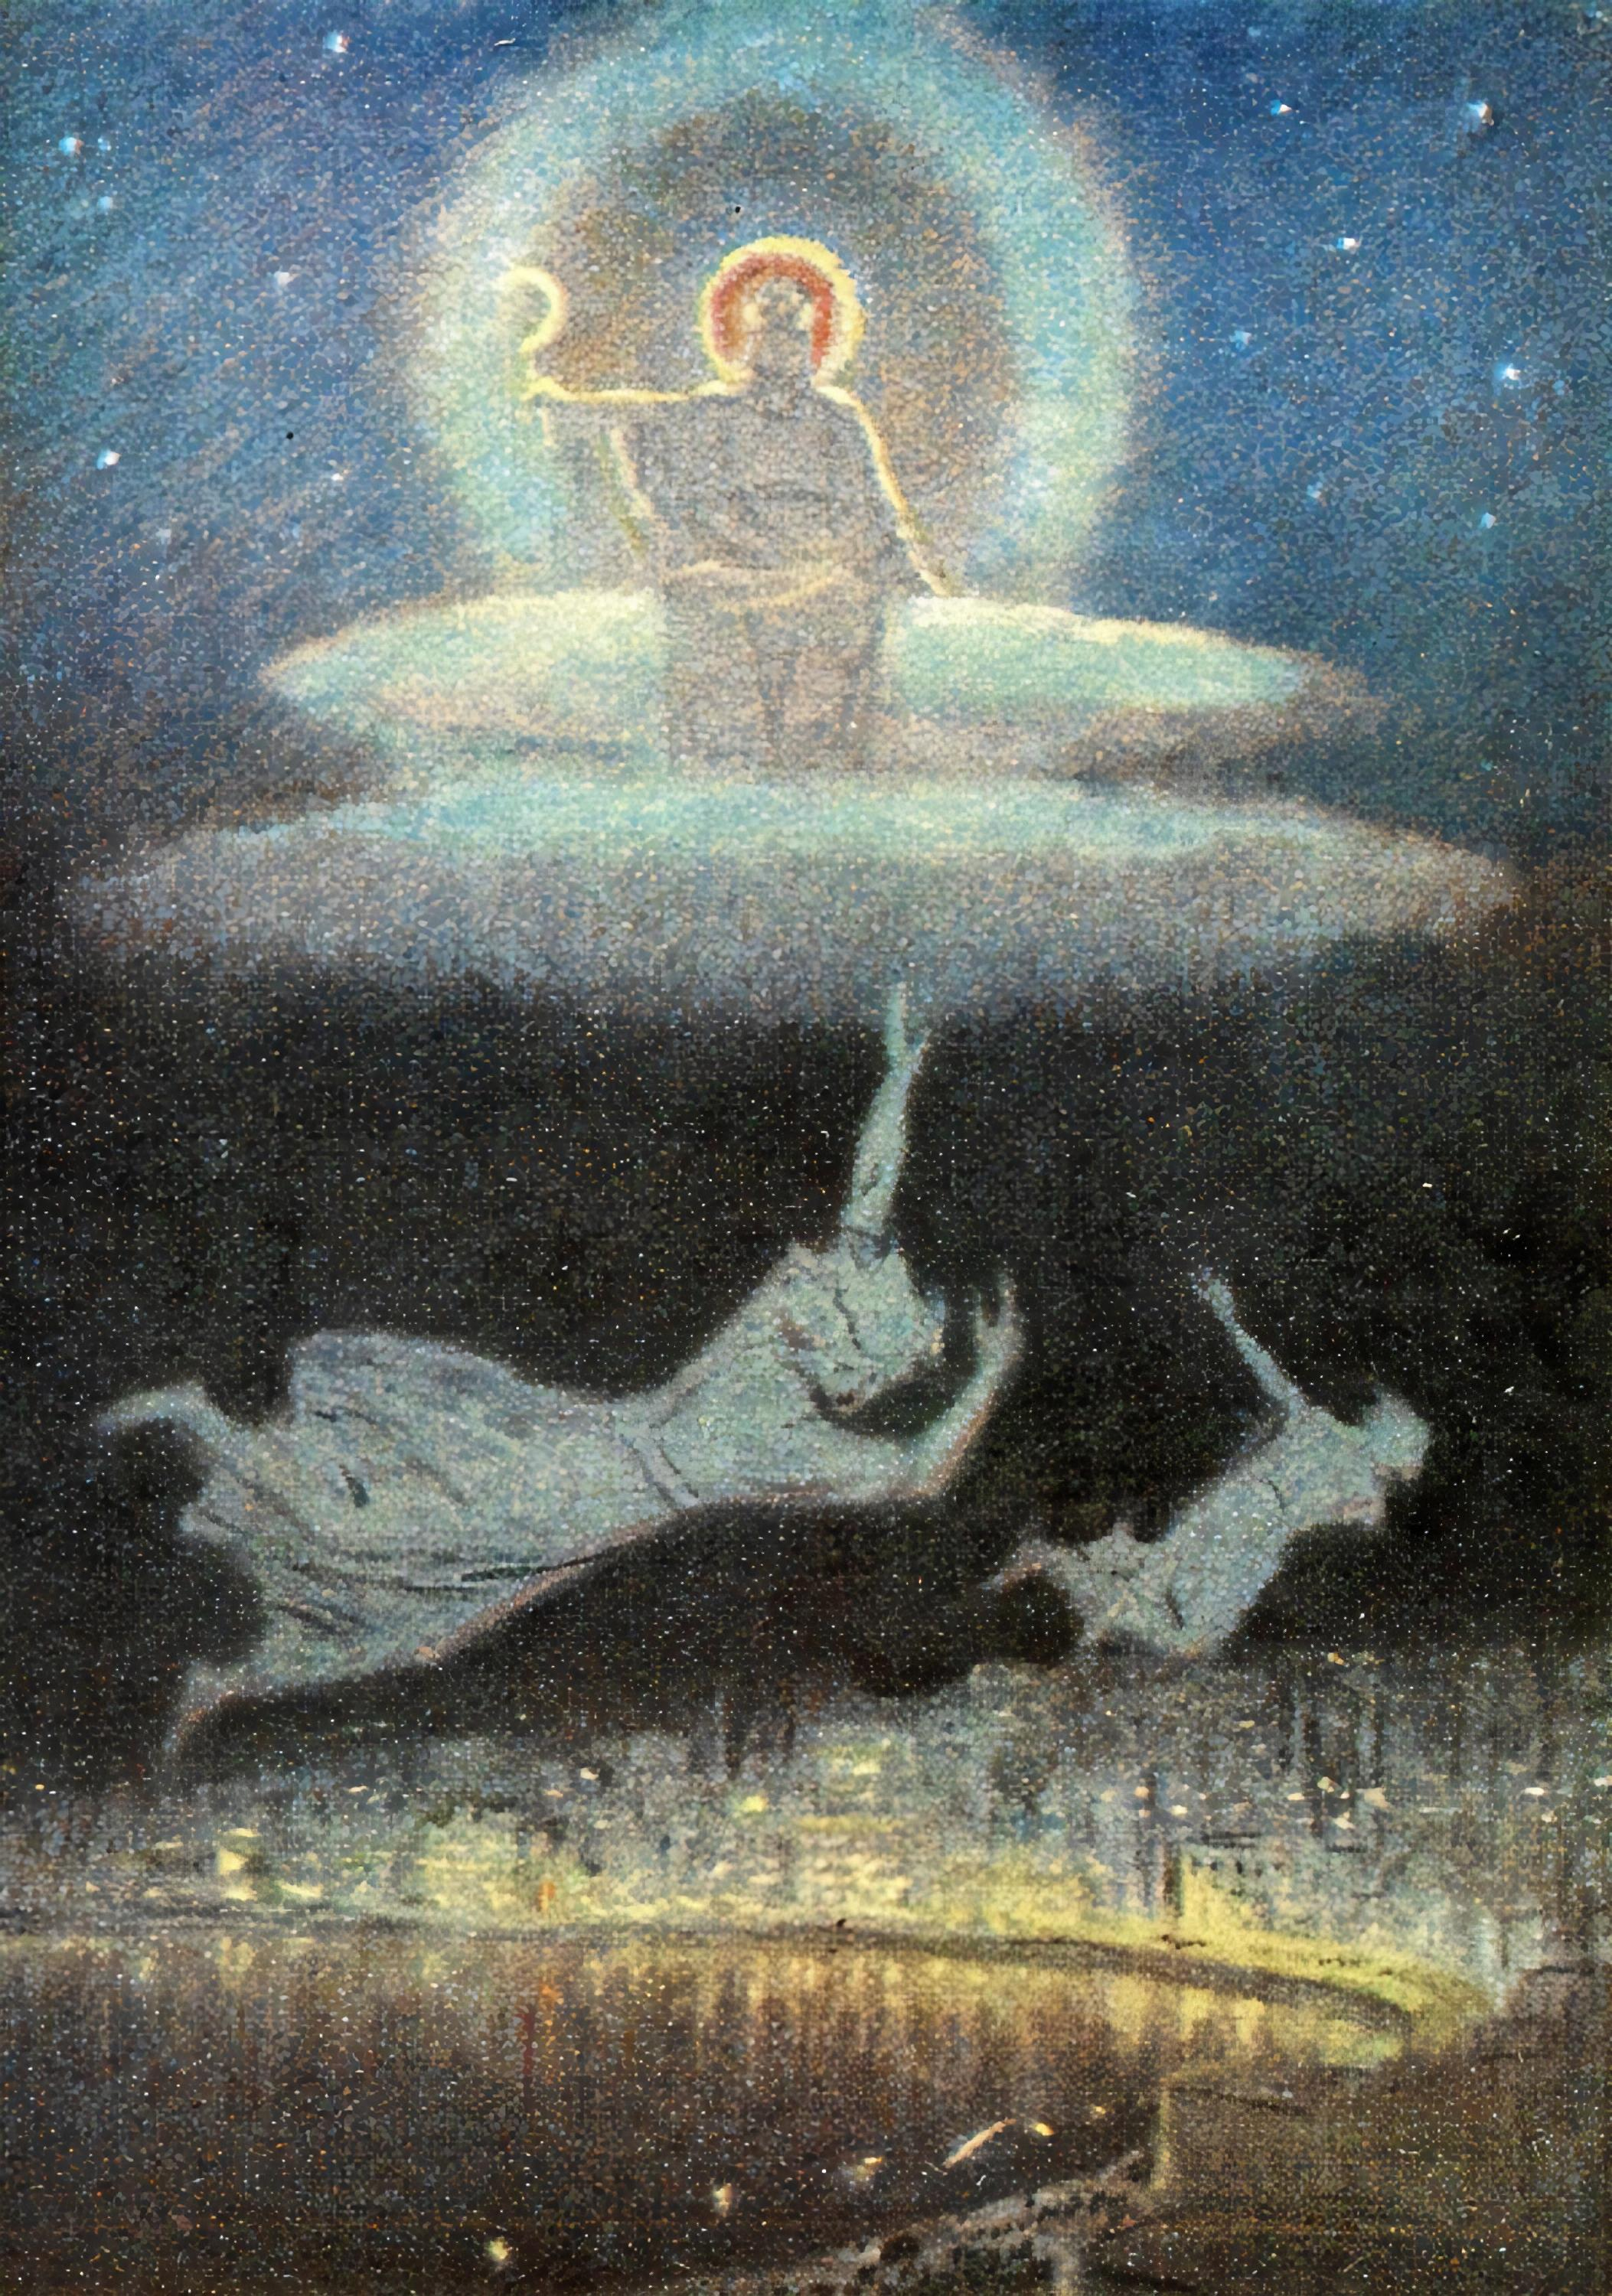
\includegraphics[width=1\textwidth]{images/illustrations/fugelgericht}
\end{center}